\documentclass[a4paper, 12pt, one column, aas_macros]{article}

%% Language and font encodings. This says how to do hyphenation on end of lines.
\usepackage[english]{babel}
\usepackage[utf8x]{inputenc}
\usepackage[T1]{fontenc}
\usepackage{aas_macros}

%% Sets page size and margins. You can edit this to your liking
\usepackage[top=1.3cm, bottom=2.0cm, outer=2.5cm, inner=2.5cm, heightrounded,
marginparwidth=1.5cm, marginparsep=0.4cm, margin=2.5cm]{geometry}

%% Useful packages
\usepackage{graphicx} %allows you to use jpg or png images. PDF is still recommended
\usepackage[hyphens]{xurl}
\usepackage[colorlinks=False]{hyperref} % add links inside PDF files
%\usepackage{breakurl}
\usepackage{amsmath}  % Math fonts
\usepackage{amsfonts} %
\usepackage{amssymb}  %
\usepackage[section]{placeins} % Add float barrier at start of each new section

%% Citation package
\usepackage[authoryear]{natbib}
\bibliographystyle{abbrvnat}
\setcitestyle{authoryear,open={(},close={)}}


\title{Exploring Procedural Generation Algorithms in \\Unity 2D}
\author{Ryan Overbeck}

\begin{document}
\maketitle


\tableofcontents


\section{Introduction}
Add introduction here
% One or two paragraphs here

\section{Binary Space Partitioning Approach}
\begin{quote}
  \emph{"A binary space partition takes a given space and splits it in half, and then takes the two areas that were created and splits those in half, and repeats until some threshold is reached."}
  \cite[p.~293]{ShortAdams2017}
\end{quote}

This quote sums up our first approach to procedurally generate rooms for our 2D dungeon. In this implementation, we define a rectangular region---the entire dungeon area---and iteratively subdivide it into smaller rectangles (potential ``rooms'') until no further meaningful subdivision is possible Lastly, some offset is applied to create space between these rooms. The following outlines how this simplified Binary Space Partitioning (BSP) approach is handled in our Unity project.

\subsection{Setting up the Initial Partition}
The process begins by defining a single large bounding area using a \texttt{BoundsInt} structure. As noted in the Unity documentation, the \texttt{BoundsInt} structure ``represents an axis aligned bounding box with all values as integers'' \citep{unity_docs}. This is useful for several reasons, among them since \texttt{BoundsInt} uses integer coordinates, it aligns naturally with tile-based systems (where tiles or grid cells are also defined by integral x, y positions).

Next, this bounding area is enqueued in a \texttt{Queue<BoundsInt>} which manages partitions that still need to be processed. A queue-based approach was selected to keep the partitioning logic simple and easy to follow. A stack-based approach would have worked equally as well---only changing the order of processing.

\subsection{Iterative Subdivision}
While there are partitions in the queue:
\begin{itemize}
  \item Dequeue the next partition.
  \item Check if the current partition meets or exceeds the \emph{minimum width} (\texttt{minWidth}) and \emph{minimum height} (\texttt{minHeight}) constraints.
  \item If it can be subdivided, choose randomly whether to \emph{prefer a horizontal} or \emph{vertical} split (a 50/50 chance). Attempt to partition the space along that orientation if there is sufficient size to do so at least twice (e.g., if the height is at least \texttt{2 * minHeight} for a horizontal split).
  \item If the chosen orientation is not feasible, try the alternative orientation.
  \item If neither orientation is possible (the partition is too small), mark that partition as finalized (a ``room'') and add it to the \texttt{partitions} list.
\end{itemize}

\subsection{Managing Subdivisions}
The actual subdivision is performed in two helper methods, \texttt{PartitionHorizontally} and \texttt{PartitionVertically}. These methods randomly determine a \emph{split point} within the valid range and create two new \texttt{BoundsInt} objects representing the subdivided spaces. Each new partition is enqueued for further subdivision if possible.

\begin{itemize}
  \item \emph{Horizontal Partition:} Splits along the y-axis, producing a top and bottom rectangle.
  \item \emph{Vertical Partition:} Splits along the x-axis, producing a left and right rectangle.
\end{itemize}

By alternating or randomly selecting horizontal versus vertical splits, the algorithm produces layouts of different shapes, preventing overly predictable results.

\subsection{Applying Offset}
TODO

\section{Random Walk Approach}
\begin{quote}
  \emph{"Random walks are produced by starting at a given point and then taking steps in random directions. Many natural processes, like molecular  motion, can be described by random walks, and they can be useful for  generating all sorts of naturalistic paths and features."}
  \cite[p.~286]{ShortAdams2017}
\end{quote}

This quote sums up our second approach to procedurally generate rooms for our 2D dungeon. In this implementation, we choose a starting position and perform a defined number of ``walks,'' each consisting of a certain number of steps. Every time we move to a new position, we record that position in a set of coordinates. After all walks are completed, these coordinates form the layout of our dungeon floor. The following outlines how this is handled in our Unity project.

\subsection{Initial Conditions}
A \texttt{HashSet} is initialized to keep track of every visited position (avoiding duplicates).

\subsection{Iterations (Walks)}
The number of iterations (walks) is determined by an input parameter. For each walk:
\begin{itemize}
  \item A \texttt{Vector2Int} for storing the previous position is set to the start position (provided by an input parameter).
  \item Perform a fixed number of steps, where each step is taken in a randomly chosen direction (up, down, left, or right). The new position after each step is added to the set, and the previous position is updated.  
\end{itemize}

\subsection{Results}
After all walks and steps are completed, the algorithm returns the set of all unique positions visited during the random walk. This collection of positions is used to place the floor tiles. The resulting dungeons will tend to have a more organic winding layout, in contrast to those resulting from the binary space partitioning (BSP) approach with its more methodical grid-like arrangement.

\section{Wave Function Collapse Approach}
The Wave Function Collapse (WFC) algorithm, specifically the Simple Tiled variant is a procedural generation method that draws inspiration from quantum mechanics to create tile-based patterns. It works by assigning a set of potential states to each tile and then progressively reducing these possibilities based on constraints from adjacent tiles, much like the collapse of a quantum state into a definite outcome. 

A simplified version of this algorithm forms the third approach for generating the layout of our dungeon. Its implementation in our Unity project is explored below.

\subsection{Setting up - Adjacency Constraints}
The first step in setting up the algorithm is to establish valid tile adjacencies for the supplied tileset. To ensure the tiles tile appropriately, every pixel on the edge of neighboring tiles must be the same color (see figure \ref{fig:wfc-tile-adjacency-constraints}). To that end, the method \texttt{GetTilesEdgesColors} accepts a list of tiles which are of the type \texttt{Texture2D} (representing bitmaps), it then extracts and returns the color information for every pixel on each tile's edge.

\begin{figure}[htbp]
  \centering
  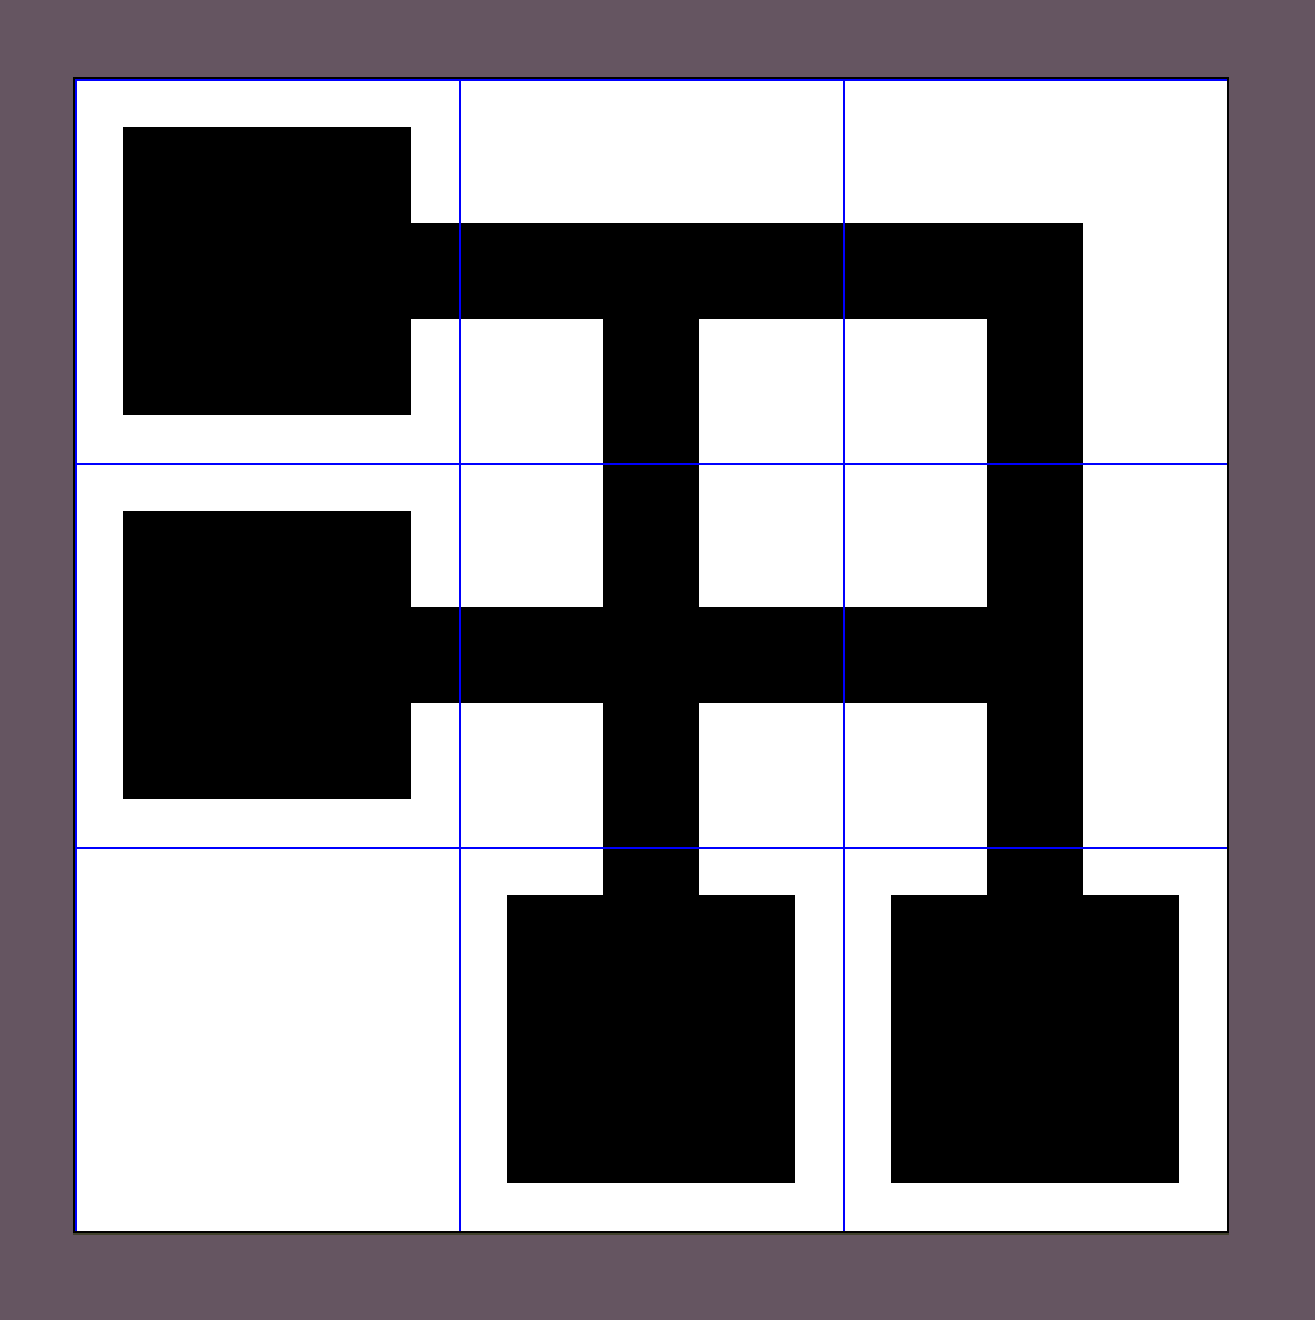
\includegraphics[width=0.7\textwidth]{images/wfc-tile-adjacency-constraints.png}
  \caption{Tile Adjacency Constraints}
  \label{fig:wfc-tile-adjacency-constraints}
\end{figure}

\subsection{Setting up - Finding Viable Tiles for each Tile's Edge}
The next step is to determine which tiles satisfy the adjacency constraints of every tile. The method \texttt{GetTilesEdgesViableTiles} performs this task by iterating through each tile and examining every one of its four edges. For each edge, the method identifies its complementary edge (i.e., the bottom edge is compared with the top edge, and the left edge with the right edge) using a helper function \texttt{GetComplementaryEdge}.

The method then compares the colors of the current edge with the corresponding complementary edge of every tile by using a pixel-by-pixel comparison via the \texttt{EdgesMatch} helper function. If the two edges match exactly, the index of the candidate tile is recorded as a viable neighbor. This process results in a three-dimensional array where each element contains the list of tile indices that can be placed adjacent to a given tile on a specific edge.

This step is crucial as it ensures that only tiles with matching edge colors are considered for adjacent placement, thus maintaining the seamless appearance of the tiled pattern.

\subsection{Setting up - Initializing the Output Grid}
TODO

\section{Difficulties}
\subsection{Challenges in Adapting WFC to Unity}
The Wave Function Collapse (WFC) algorithm offers an innovative approach to procedural content generation. However, adapting it to a Unity 2D project presented several challenges, primarily due to shortcomings in the primary reference, the source for it on GitHub. \cite{mxgmn}

A major source of difficulty was the repository’s README, which conflates two distinct variants of the algorithm: \emph{Simple Tiled} and \emph{Overlapping}. The failure to clearly differentiate between these variants led to confusion in the description of the algorithm which was crucial for reasoning about the source code due to poor naming conventions, lack of inline documentation, and terminology borrowed from Quantum Mechanics despite a tenuous connection.

This was not a unique difficulty, as one researcher noted, ``in personal correspondence with several users of WFC, we learned that many of them treated the code as a black box''. \citep{karth}


\subsection{Challenges in Moving to Tile Generation Over Time}
When the project first aimed to generate a dungeon floor, the tile placement occurred synchronously on \texttt{Start()}. This approach was straightforward to implement but lacked any concept of observable progression over time. Addressing this necessitated several changes. 

First, the original data structure for storing the positions of the floor tiles, a \texttt{HashSet} needed to be changed so that order could be preserved. Using a \texttt{Queue} was necessary to maintain first-in-first-out order. However, this change introduced a new challenge: since a \texttt{Queue} alone does not handle duplicates, a separate \texttt{HashSet} had to be used in parallel to record visited positions. By checking against this \texttt{HashSet} before enqueueing a new coordinate, the system could retain an ordered structure while still preventing repeated tiles from being added. Note that while Unity's \texttt{Tilemap.SetTile} method can handle duplicates it would obfuscate how the room is constructed over time so it became necessary to deal with them here. 

Second, switching from a synchronous approach to an incremental, time-based approach introduced the need for coroutines. Previously, the entire tile set could be drawn in a single loop, effectively blocking until all positions were placed. In contrast, placing one tile every half-second requires the code to yield partway through execution so that the game loop can continue running. Implementing the coroutine \texttt{DrawFloorTilesOverTime} allowed each tile placement to be spaced out over time without freezing the entire game.

Third, as tiles were placed over time, it became important to communicate the dungeon generation’s progress to the player. A simple UI element was introduced to display both the total number of tiles to be placed and the number of tiles already placed, updating in real time as new positions were set.

\begin{figure}[htbp]
  \centering
  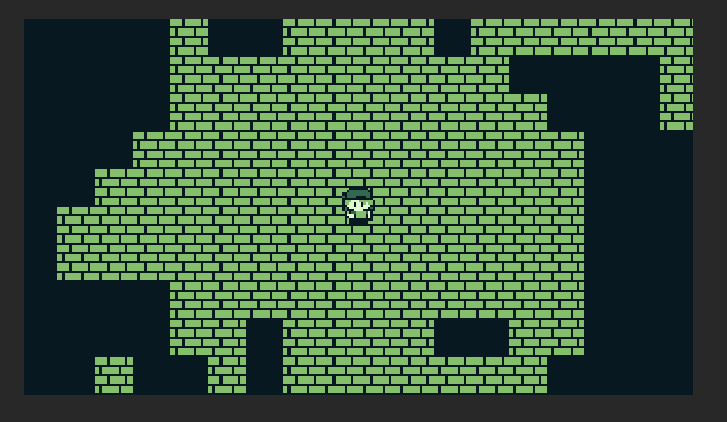
\includegraphics[width=0.7\textwidth]{images/difficulty-1-before.png}
  \caption{Challenge 4.1 - game view before}
  \label{fig:difficulty-1-before}
\end{figure}

\begin{figure}[htbp]
  \centering
  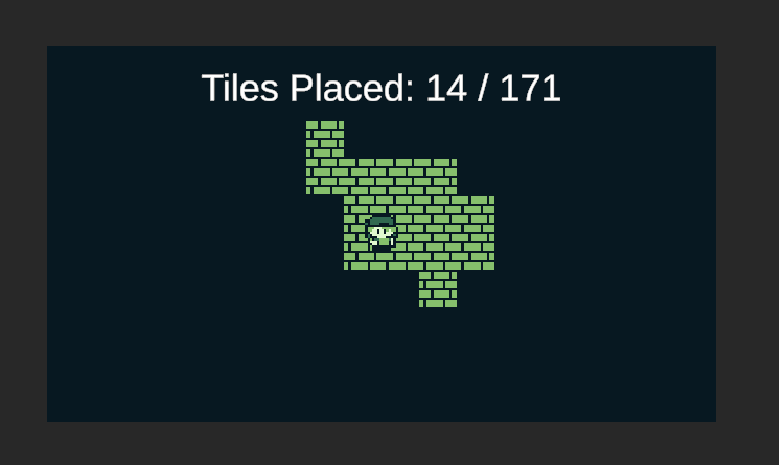
\includegraphics[width=0.7\textwidth]{images/difficulty-1-after.png}
  \caption{Challenge 4.1 - game view after}
  \label{fig:difficulty-1-after}
\end{figure}

\section{Impact of Previous Courses on Project}
\subsection{CSCI 451 and Utilizing Unity Coroutines}
Threads in C\# represent an operating-system-level construct. As stated by Silberschatz \emph{et al.}, ``A thread is a basic unit of CPU utilization; it comprises a thread ID, a program counter, a register set, and a stack'' \cite{silberschatz}. This means that each thread is scheduled independently by the operating system and can take advantage of multiple processor cores for true parallelism. However, the creation and management of multiple threads can be resource-intensive, and programmers must carefully manage data shared between threads to avoid race conditions. 

Unity coroutines, on the other hand, are not scheduled by the operating system. They are functions ``that can be suspended, resumed, and executed cooperatively (often on the same thread)'' \cite{nosenko}. In Unity, coroutines primarily run on the main thread and yield control voluntarily, allowing the engine to manage when to resume them. This cooperative model avoids the complexity of thread synchronization, but it does not offer true parallelism by default. Coroutines are particularly useful for tasks that must be broken into incremental steps across frames, such as animations or in the case of this project, long-running operations where you do not want to block the main thread.

My understanding of these concurrency mechanisms was greatly enhanced by taking \textit{CSCI 451 Operating Systems}. The course covered core concepts of processes, threads, synchronization, and CPU scheduling, providing the theoretical background to appreciate how the operating system manages threads and why threads are relatively expensive compared to language-level, cooperative concurrency mechanisms like coroutines. By exploring concurrency at the OS level first, it enables deeper insight into how coroutines abstract these complexities and thus offer a simpler model for many game development scenarios.

\subsection{WRIT 102 and Academic Sourcing/Technical Writing}
In addition to technical courses, the project benefited significantly from the skills acquired from University Studies, such as \textit{WRIT 102 Introduction to Academic Writing}. This course, which emphasized careful analysis, systematic research, and the construction of coherent academic arguments laid a solid groundwork for both identifying credible resources and organizing the paper effectively.

The techniques learned in \textit{WRIT 102} proved instrumental during the research phase by facilitating the systematic identification and evaluation of academic sources that supported the project. Moreover, the course’s focus on proper documentation and citation ensured that all referenced materials were integrated seamlessly and accurately, thereby maintaining the academic integrity of the paper.

Lastly, the critical reading and persuasive writing strategies honed in the course helped in articulating complex technical concepts clearly and persuasively, bridging the gap between technical content and academic presentation.

\section{Conclusion}

\bibliography{references}
\end{document}